\section{Robust solution: SRP-PHAT}
\subsection{Behavior and error sources}
\subsubsection{Array response}
Beamforming techniques for sound localization have been study intensively over the last decades. The main drawback of the conventional beamforming are the side lobes in the localization results. If SRP-PHAT algorithm is applied to a tetrahedral array and cross-correlations values at different delays are summed by the beamformer (Eq. \ref{eq:srpSum}), subsidiary peaks can appear in the energy map at DOAs that don't correspond to the incident plane wave DOA. Those peaks in the SRP-PHAT energy map can mask real sources or even add up to other peaks from other sources, thus display a fake source. Deconvolution methods remove those peaks to reveal the correct peak. The algorithms for deconvolution are based on the point spread function, which is the response of the array to a point source. 
%For far-field, this means a plane wave incident with a particular DOA on the microphone array. In transfer function terms, the array response is `deconvolved' from the final energy map. 
%While this problem has motivated the creation of new beamformers {!!CITATION!!}, the problem lies in the method itself.
%New classes of algorithms have been developed to deconvolve the noise signals from the desired steered signal such as CLEAN \cite{sijtsma2007clean} and DAMAS \cite{brooks2006deconvolution}.
%DAMAS was acknowledged a major breakthrough in array processing. At first research was mainly focused on aeroacoustic for the development of near-field sound localization system but it seems that a new enthusiasm has taken over scientists trying to solve other sound localization problems. 
%While the DAMAS method is mainly designed for near field measurements in the range of the array aperture size, a new deconvolution method has been proposed [\cite{zhao2015large}, \cite{zhao2017large}] where a small aperture array is used to measure source signal in the far field. The principle behind point spread function is discussed in the following section. Then a review of the underlying principles of the main deconvolution algorithms is given, and finally a specific method for coherent and incoherent sources localization is discussed.
A perfect array will detect a point precisely at the actual source location and nothing elsewhere. This, however, is not the general case. For example, given a single pair of microphones, and assuming far-field incidence, the only information that can be concluded from a single point source is the angle of incidence on the array. This angle is a vector combination of source azimuth and elevation. This leads to a circle around the array where the source might be located (circular maximum peak). This circle is the base of the cone resulting from the cone approximation discussed previously.
%\begin{figure}[H]
%    \centering
%    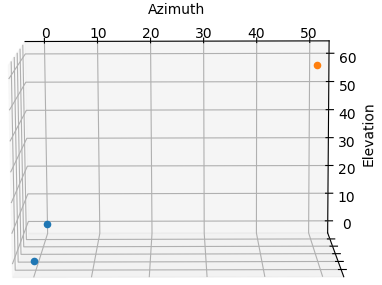
\includegraphics[width=0.98\textwidth]{Figures/2mic1src.png}
%    \caption{Figure depicts a source located at $50\degree$ azimuth and $60\degree$ elevation (orange dot). Two microphones (blue dots) will be used to localize the source.}
%    \label{fig:2mic1srcPos}
%\end{figure}
\begin{figure}[H]
    \centering
    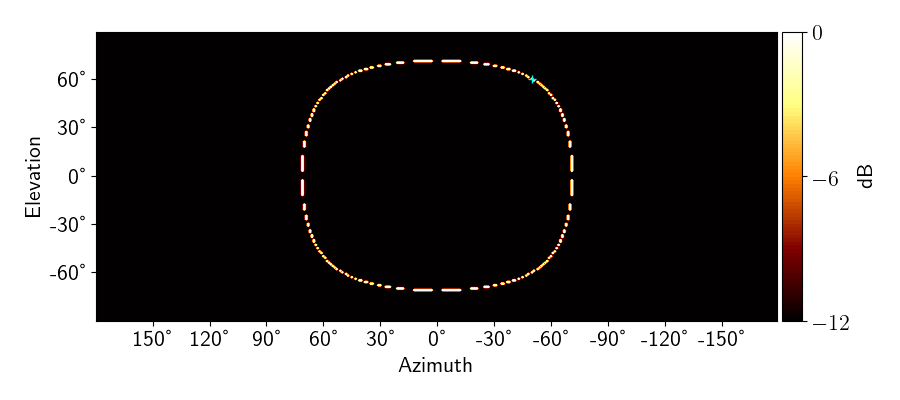
\includegraphics[width=0.8\textwidth]{Figures/2mic1srcRes.png}
    \caption{SRP-PHAT is run to localize a single point source with 2 microphones. The source is localized to a circle. The blue cross indicates the actual source location.}
    \label{fig:2mic1src}
\end{figure}
If three microphones are placed in a horizontal equilateral triangle, we get three circles (three possible pairs of microphones) from localization. The maximum peak occurs at 2 locations with azimuth=50$\degree$ and elevation=$\pm 60\degree$.
\begin{figure}[H]
    \centering
    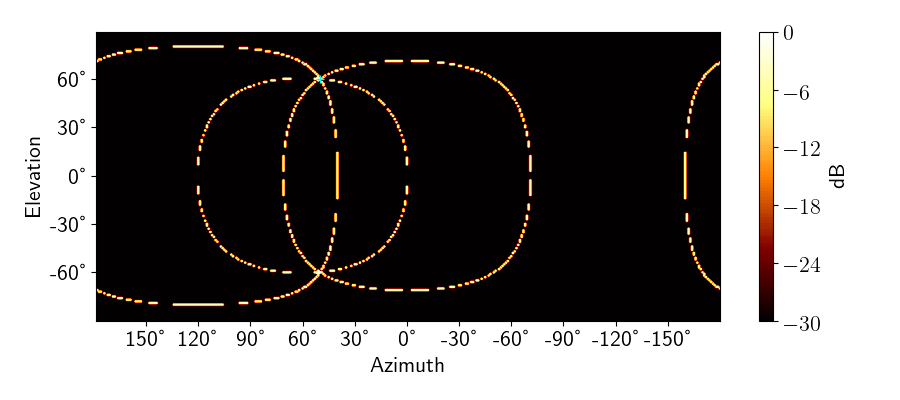
\includegraphics[width=0.8\textwidth]{Figures/3mic1srcRes.png}
    \caption{SRP-PHAT is run to localize the source with 3 microphones.}
    \label{fig:3mic1src}
\end{figure}
For a tetrahedral array, the point spread function is a combination of circles from the 6 possible microphone pairs. This time the main peak occurs at exactly one point. However, since only 3 pairs out of the 6 are linearly independent (Eq. \ref{Eq:linearDep}), the localization should really be done considering only 3 of those pairs. The result in shown in fig. \ref{fig:4mic1srcInd}.
\begin{figure}[h]
    \centering
    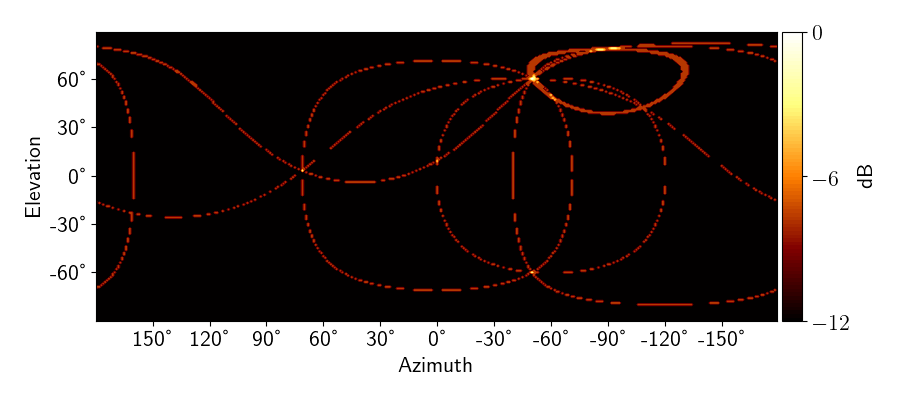
\includegraphics[width=0.8\textwidth]{Figures/4mic1srcRes.png}
    \caption{SRP-PHAT is run to localize the source with a tetrahedral array.}
    \label{fig:4mic1src}
\end{figure}
\begin{figure}[h]
    \centering
    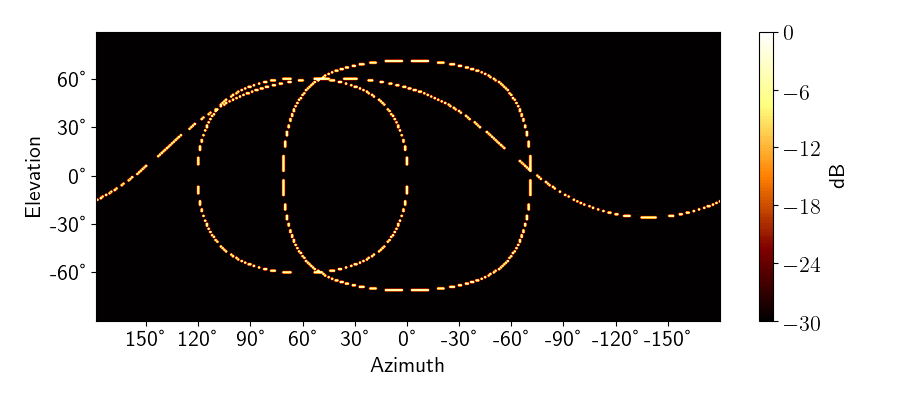
\includegraphics[width=0.8\textwidth]{Figures/Ind4mic1srcRes.png}
    \caption{SRP-PHAT is run to localize the source with a tetrahedral array but only linearly independent microphone pairs are considered}
    \label{fig:4mic1srcInd}
\end{figure}
Considering only independent microphones, Eq. \ref{eq:srpSum} can be rewritten as, 
\begin{equation}
    S_{SRP}(\theta,\phi)=\sum\limits_{i=1}^{M-1}{R_{x_0,x_i}[f_{0,i}(\theta,\phi)]}
     \label{eq:srpSumInd}
\end{equation}
\subsubsection{Effect of noise}
The result in fig. \ref{fig:4mic1srcInd} is applicable only in ideal conditions (zero noise, no reflections and perfectly planar propagation). The localization result for noisy conditions is depicted in fig. \ref{fig:4mic1srcNoisy}. As expected, the performance deteriorates as the SNR drops. 
\begin{figure}[H]
\begin{subfigure}[b]{0.96\textwidth}
    \centering
    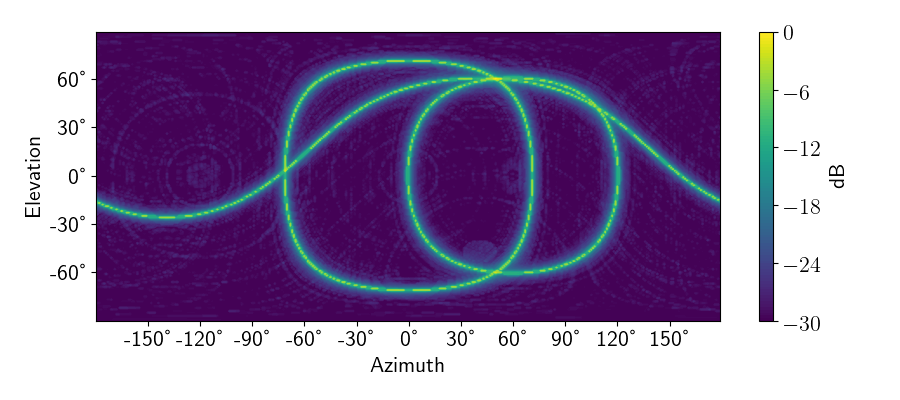
\includegraphics[width=0.8\textwidth]{Figures/Ind4mic1srcRes20.png}
\end{subfigure}
\vskip \baselineskip
\begin{subfigure}[b]{0.96\textwidth}
    \centering
    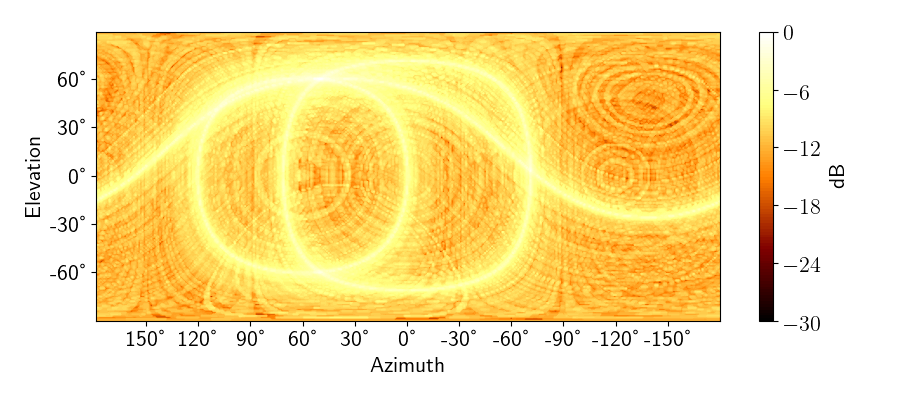
\includegraphics[width=0.8\textwidth]{Figures/Ind4mic1srcRes0.png}
\end{subfigure}
\vskip \baselineskip
\begin{subfigure}[b]{0.96\textwidth}
    \centering
    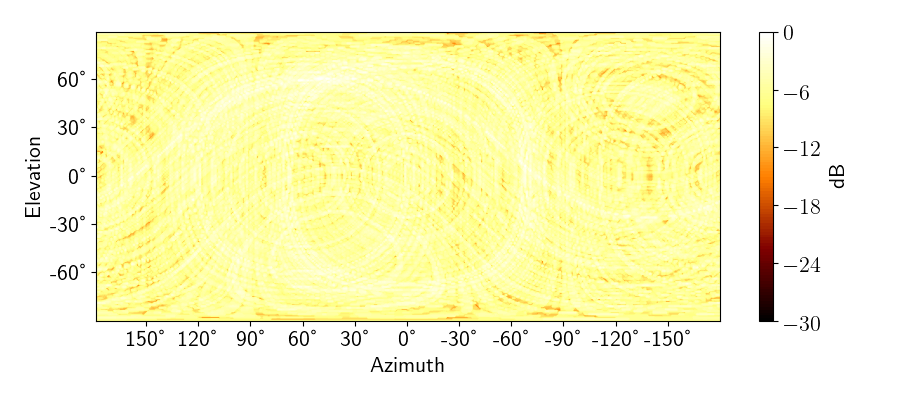
\includegraphics[width=0.8\textwidth]{Figures/Ind4mic1srcResNeg10.png}
\end{subfigure}
\caption{Figures depict from top-to-bottom SRP-PHAT localization results with SNR = 20dB, SNR = 0dB, SNR = -10dB}
\label{fig:4mic1srcNoisy}
\end{figure}
\subsubsection{Effect of temperature}
Temperature affects the speed of sound and thus affects the delay time between the microphone pairs. During measurement, if it is assumed to be room temperature, this could lead to errors in the localization results. Fig.\ref{fig:4mic1srcTemp} depicts the effect of temperature on localization results, where wave files received by the tetrahedral microphone array at temperatures of $0\degree C$, $20\degree C$ and $-40\degree C$ are simulated. Then the localization is run assuming the speed of sound to be 343m/sec in every case. The figure shows zoomed in results around the source location. As can be seen in the figure, an error in recording temperature has the effect of `de-focusing' the main peak.
\begin{figure}[H]
    \centering
    \begin{subfigure}[b]{0.96\textwidth}
    \centering
    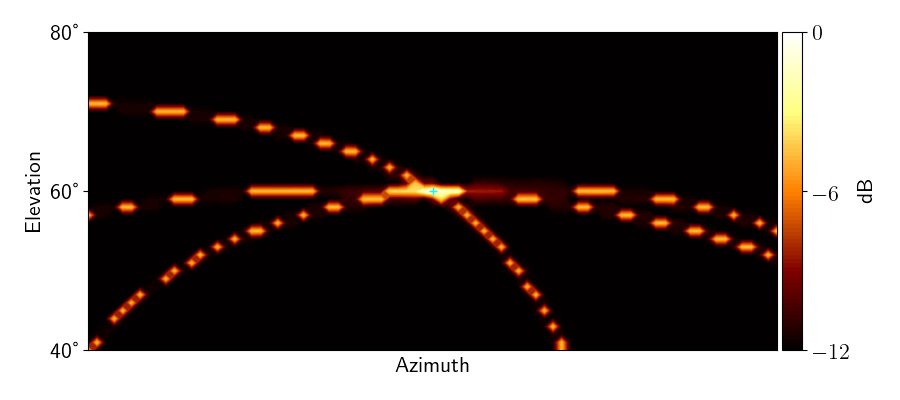
\includegraphics[width=0.8\textwidth]{Figures/Ind4mic1srcSum20deg.png}
\end{subfigure}
\vskip \baselineskip
\begin{subfigure}[b]{0.96\textwidth}
    \centering
    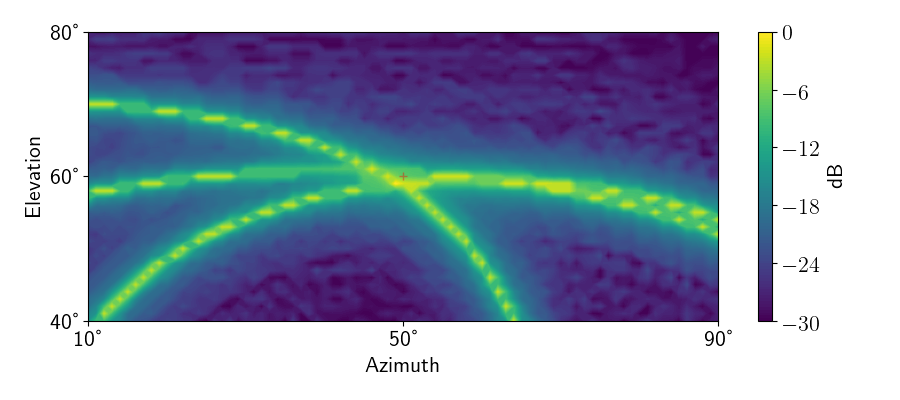
\includegraphics[width=0.8\textwidth]{Figures/Ind4mic1srcSum0deg.png}
\end{subfigure}
\vskip \baselineskip
\begin{subfigure}[b]{0.96\textwidth}
    \centering
    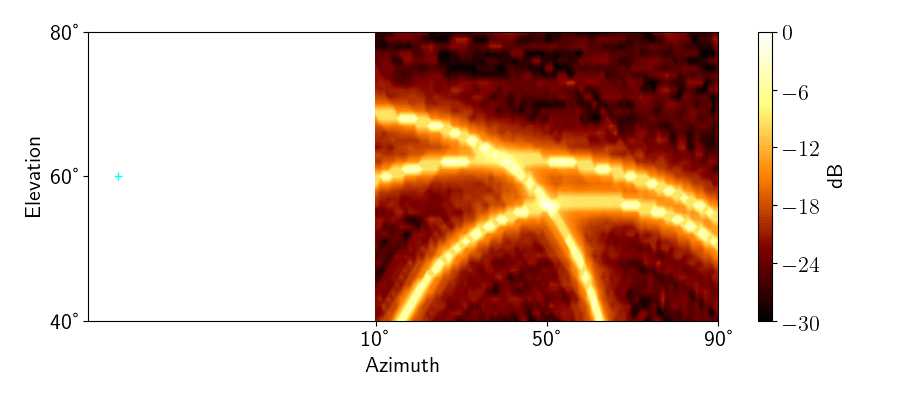
\includegraphics[width=0.8\textwidth]{Figures/Ind4mic1srcSumNeg40deg.png}
\end{subfigure}
\caption{Figures depict from top-to-bottom SRP-PHAT localization results with at temperatures of $20\degree C$, $0\degree C$ and $-40\degree C$.}
\label{fig:4mic1srcTemp}
\end{figure}
\subsubsection{Effect of wind}
Wind speed effects the speed of sound in the direction of propagation. Delays between different array pairs would be affected depending on where the SRP search is looking and from what direction the wind is blowing. If wind blows perpendicular to the direction of propagation of the sound from the source, then it does not affect the localization. Fig.\ref{fig:4mic2srcWind} depicts the effect of wind on localization results at wind of 10$m/s$ blowing at $90\degree$, $45\degree$ and $180\degree$ to a source at ($50\degree$,$60\degree$) without any wind correction. It can be seen that when wind blows at $90\degree$, it does not affect the localization results. The magnitude of error when wind blows non-perpendicular to the sound propagation direction depends on the wind speed and the degree of alignment with the wind direction.
\begin{figure}[H]
    \centering
    \begin{subfigure}[b]{0.96\textwidth}
    \centering
    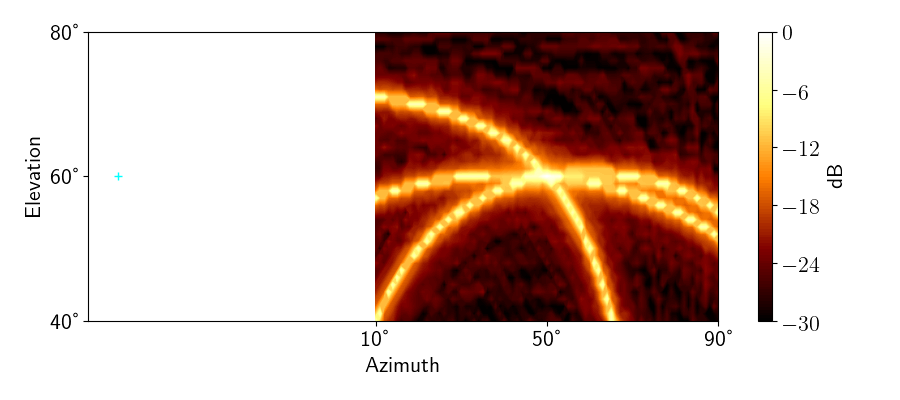
\includegraphics[width=0.8\textwidth]{Figures/4mic1srcWind90.png}
\end{subfigure}
\vskip \baselineskip
\begin{subfigure}[b]{0.96\textwidth}
    \centering
    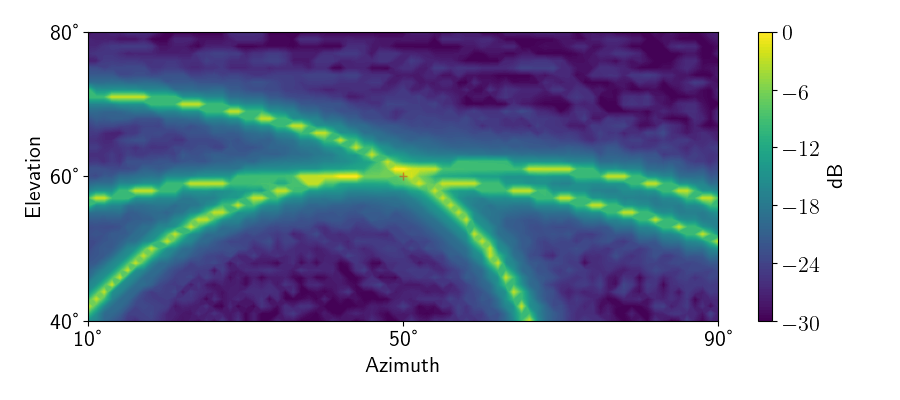
\includegraphics[width=0.8\textwidth]{Figures/4mic1srcWind45.png}
\end{subfigure}
\vskip \baselineskip
\begin{subfigure}[b]{0.96\textwidth}
    \centering
    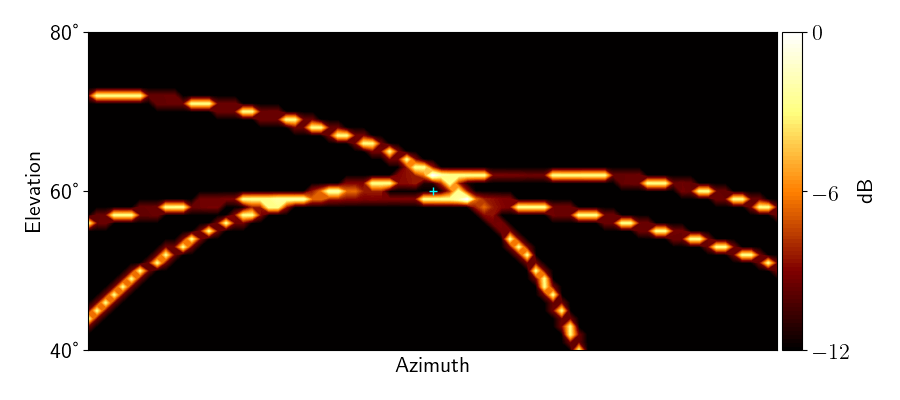
\includegraphics[width=0.8\textwidth]{Figures/4mic1srcWind45Fast.png}
\end{subfigure}
\caption{Figures depict from top-to-bottom SRP-PHAT localization results with wind of $10 m/sec$ blowing $90\degree$, $10 m/sec$ blowing $45\degree$ and $30 m/sec$ blowing $45\degree$ to the source sound propagation direction.}
\label{fig:4mic2srcWind}
\end{figure}
\subsubsection{Effect of ground reflections}
Sound received from a far-field sound source consists of the plane wave and the spherical wave component (Eq. \ref{Eq:GroundWave}). The spherical wave component creates a horizontal ground wave with the ground and quickly attenuates with distance. The plane wave creates a reflected wave with ground (image source) whose magnitude depends on the acoustic reflection coefficient of the ground material. Rudimentary simulations for a source located at $(\theta,\phi)$ can be made assuming image sound source located at $(\theta,-\phi)$. Fig. \ref{fig:4mic1srcRef} shows the localization results with source at ($50\degree$,$60\degree$) for different ground reflection coefficients. The microphone pairs in the tetrahedral array that are parallel to the ground locate both the source and the image on the same cone. This causes the image to be localized at a higher level than it actually is.
\begin{figure}[H]
    \centering
    \begin{subfigure}[b]{0.96\textwidth}
    \centering
    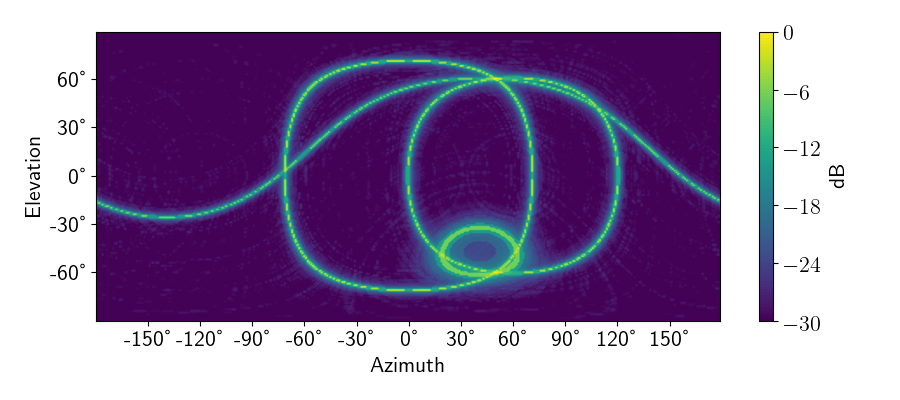
\includegraphics[width=0.8\textwidth]{Figures/4mic1srcRef100.png}
\end{subfigure}
\vskip \baselineskip
\begin{subfigure}[b]{0.96\textwidth}
    \centering
    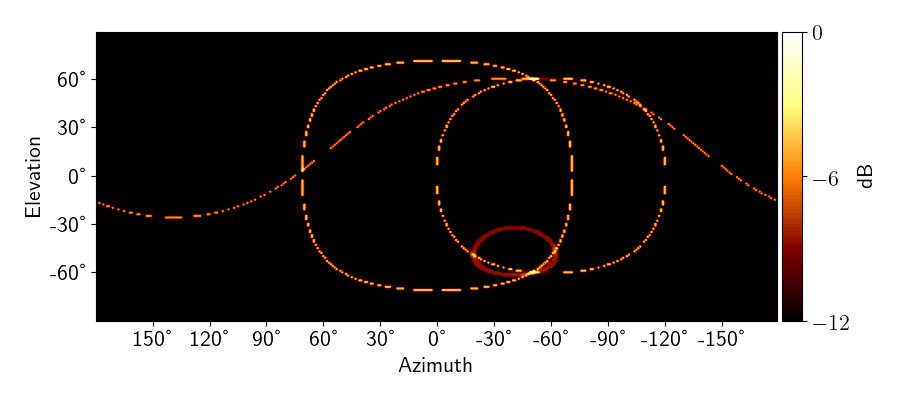
\includegraphics[width=0.8\textwidth]{Figures/4mic1srcRef60.png}
\end{subfigure}
\vskip \baselineskip
\begin{subfigure}[b]{0.96\textwidth}
    \centering
    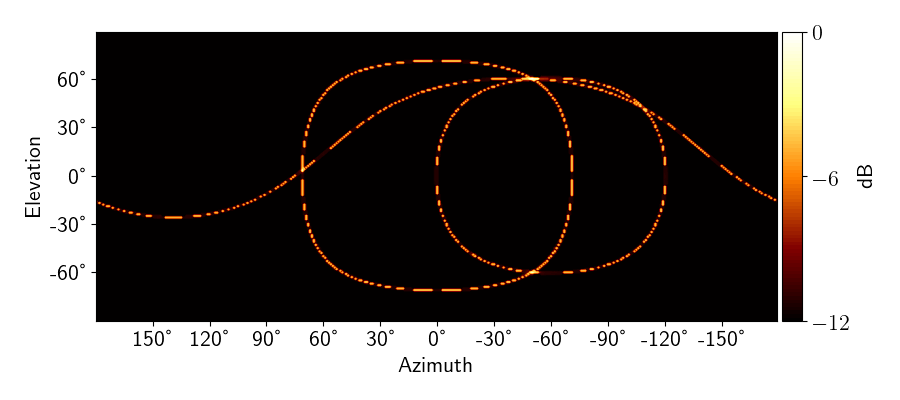
\includegraphics[width=0.8\textwidth]{Figures/4mic1srcRef10.png}
\end{subfigure}
    \caption{Figures depict from top-to-bottom SRP-PHAT localization results with ground reflection coefficients (R) of 1, 0.6 and 0.1. Even though the image source should get significantly weaker for R=0.1, it does not as it is supported by the localization cones from the real source.}
    \label{fig:4mic1srcRef}
\end{figure}
%\subsubsection{Effect of `phase' noise}
%Coming Soon!
\newpage
\subsubsection{Effect of angular resolution of localization}
Similar to the 2D angular resolution due to a single pair (Fig. \ref{fig:res_diff}), the tetrahedral array has its own 3D  angular resolution depending on the sample rate and the array aperture size. Fig. \ref{fig:res_diff_3d} describes the angular resolution of a tetrahedral array of aperture 1m for different sample rates. If the SRP search space is $360\degree$ by $180\degree$, and the resolution of search is $1\degree$, there will be some angular locations where the delay in sample between a microphone pair is fractional. For simplicity, this fractional delay is rounded for all plots in this thesis. This means that certain locations will contain duplicate data from the nearest integral delay location to themselves. Obviously, the resolution improves for higher sample rate.
\begin{figure}[H]
    \centering
    \begin{subfigure}[b]{0.96\textwidth}
    \centering
    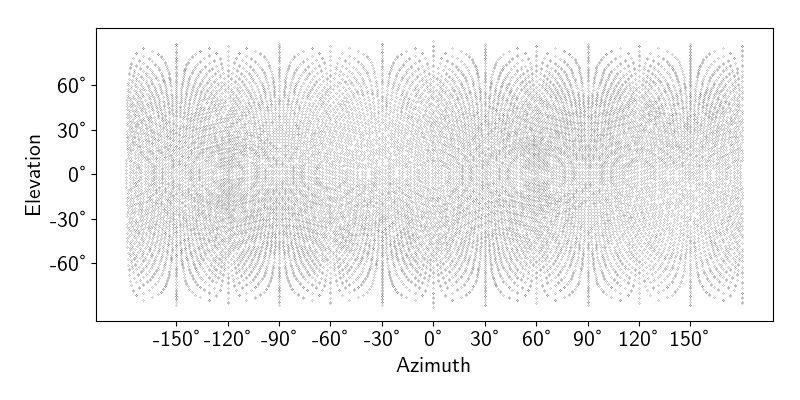
\includegraphics[width=0.7\textwidth]{Figures/res3d12k.png}
\end{subfigure}
\vskip \baselineskip
\begin{subfigure}[b]{0.96\textwidth}
    \centering
    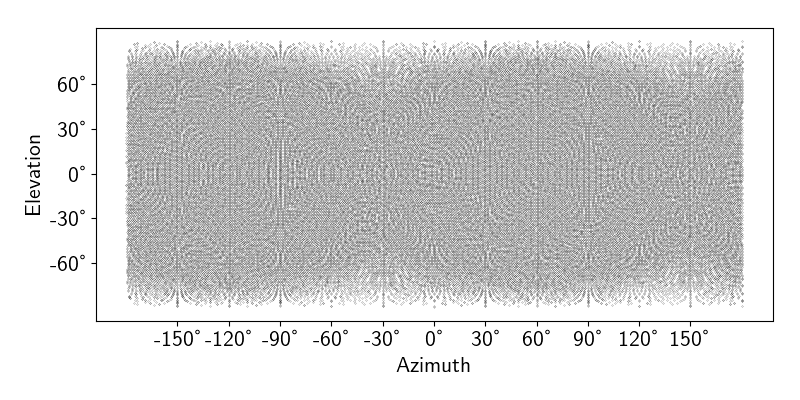
\includegraphics[width=0.7\textwidth]{Figures/res3d48k.png}
\end{subfigure}
\vskip \baselineskip
\begin{subfigure}[b]{0.96\textwidth}
    \centering
    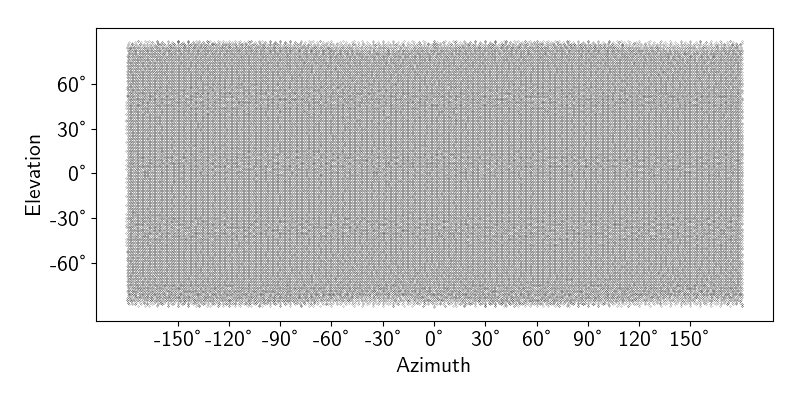
\includegraphics[width=0.7\textwidth]{Figures/res3d192k.png}
\end{subfigure}
    \caption{Figures depict from top-to-bottom SRP-PHAT angular resolution of localization with sample rate of 12kHz, 48kHz and 192kHz.}
    \label{fig:res_diff_3d}
\end{figure}
\subsubsection{Effect of change in aperture size or sample rate}
As discussed above and shown in fig. \ref{fig:res_diff}, reducing the aperture size or sample rate also reduces the angular resolution of localization, which causes a direct degradation in SRP-PHAT performance. Fig. \ref{fig:4mic1srcAper} depicts the effect of reducing sample rate or aperture size on the SRP-PHAT localization results.
\begin{figure}[H]
    \centering
    \begin{subfigure}[b]{0.96\textwidth}
    \centering
    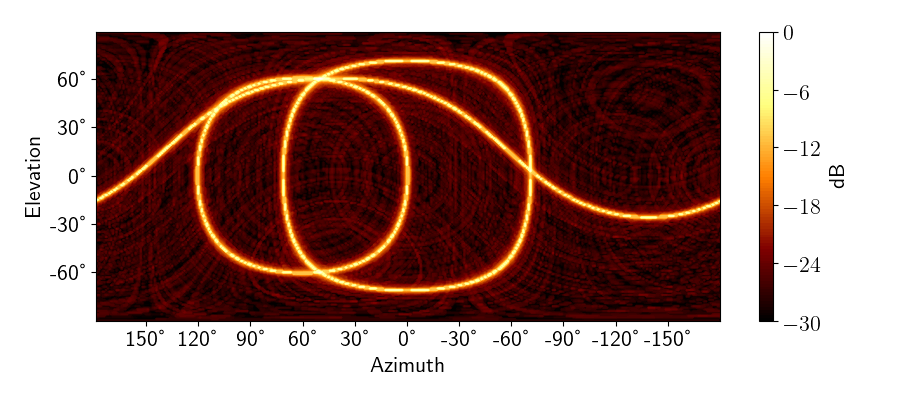
\includegraphics[width=0.7\textwidth]{Figures/Tetra1m.png}
\end{subfigure}
\vskip \baselineskip
\begin{subfigure}[b]{0.96\textwidth}
    \centering
    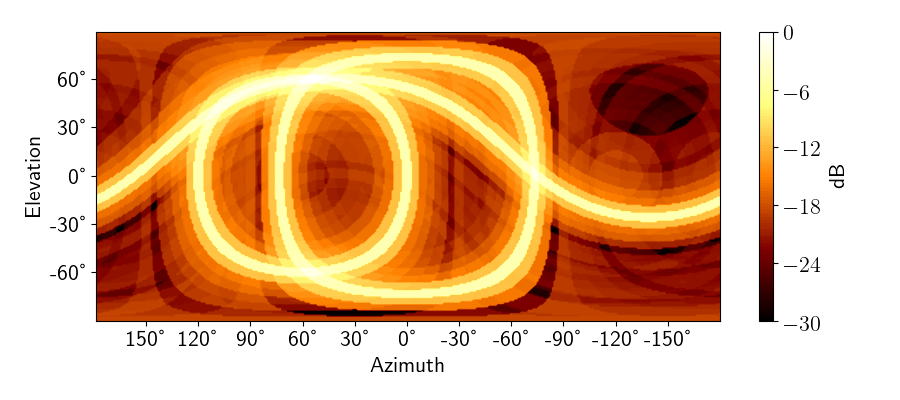
\includegraphics[width=0.7\textwidth]{Figures/Tetra10cm.png}
\end{subfigure}
\vskip \baselineskip
\begin{subfigure}[b]{0.96\textwidth}
    \centering
    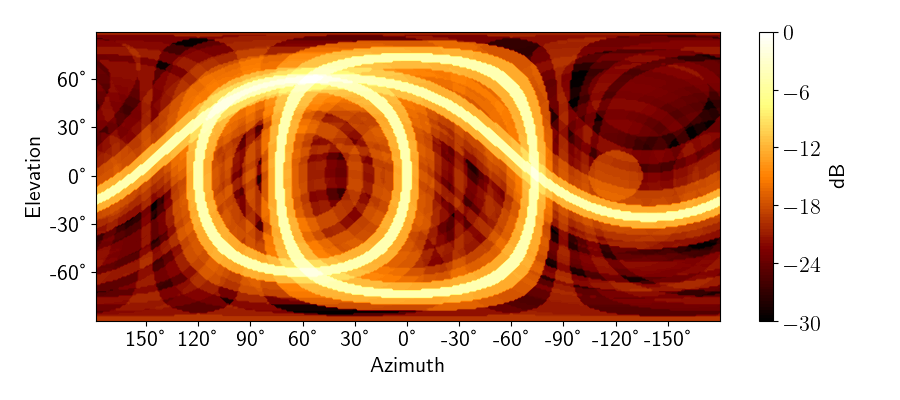
\includegraphics[width=0.7\textwidth]{Figures/Tetra1mFS.png}
\end{subfigure}
    \caption{Figures depict from top-to-bottom SRP-PHAT localization results with tetrahedral microphone array aperture size of 1m@48kHz, 10cm@48khz and 1m@4.8kHz.}
    \label{fig:4mic1srcAper}
\end{figure}
\newpage
\subsubsection{Effect of using the redundant microphone pairs}
A thing to note is that Eq. \ref{Eq:linearDep} is only true for no noise conditions. In case of low SNR, there is a potential to gain information by using the redundant microphone pairs. This is because if noise at all microphones is assumed to be uncorrelated, even though noise causes some microphone pairs to detect a source at a 'sourceless` location of the SRP search, certain microphone pairs will have a lower magnitude at that location. So in case of a SRP-PHAT, the sum of all microphone pairs will be higher at the real source location, and at other locations, the sum due to the noise will be suppressed. Fig. \ref{fig:4mic1srcRedun} shows the effect of using all microphone pairs for noisy conditions. Note that the dynamic range in the figure has been lowered to highlight the differences. It can be seen that using all the microphone pairs adds to the overall noise as more pairs can now contribute to the SRP sum, however, ideally the peak of the true source would also be higher, due to more pairs providing power at the source location. 
\begin{figure}[H]
\begin{subfigure}[b]{0.96\textwidth}
    \centering
    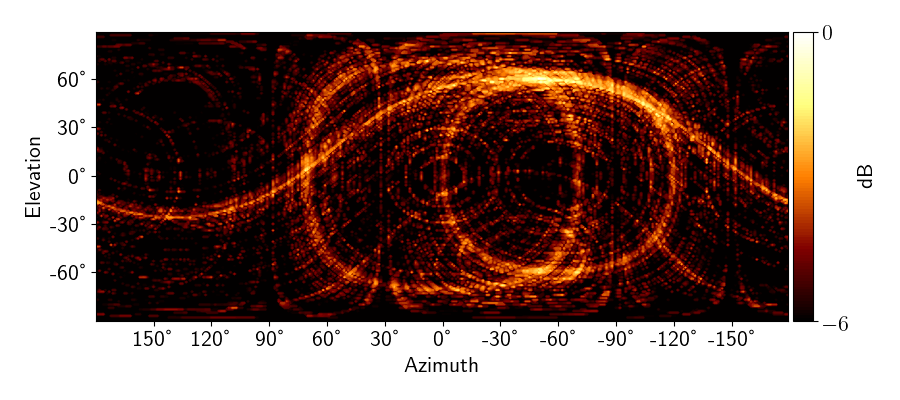
\includegraphics[width=0.8\textwidth]{Figures/Ind4mic1srcResNeg10LowDyn.png}
\end{subfigure}
\vskip \baselineskip
\begin{subfigure}[b]{0.96\textwidth}
    \centering
    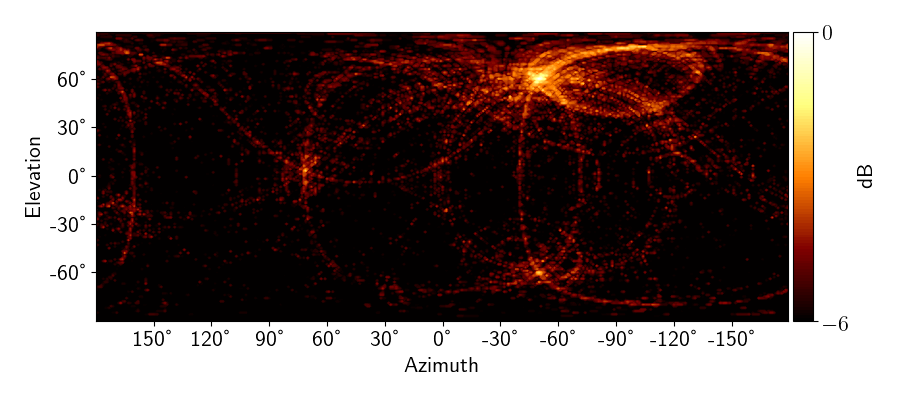
\includegraphics[width=0.8\textwidth]{Figures/Dep4mic1srcResNeg10LowDyn.png}
\end{subfigure}
\caption{Figures depict from SRP-PHAT localization results with SNR = -10dB, for independent microphone pairs (top), and for all  microphone pairs (bottom)}
\label{fig:4mic1srcRedun}
\end{figure}
%\subsubsection{Effect of adding more microphones}
%It is of interest to test the scalability of the algorithm by adding more microphones. Theoretically, adding microphones should add independent pairs and thus lower the noise floor (normalized) to improve results in a low SNR scenario. 
%\begin{figure}[H]
%\begin{subfigure}[b]{0.96\textwidth}
%    \centering
%    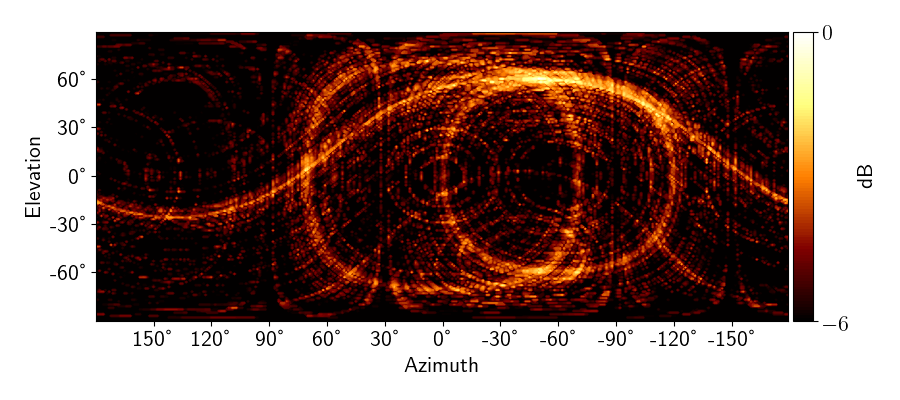
\includegraphics[width=0.8\textwidth]{Figures/Ind4mic1srcResNeg10LowDyn.png}
%\end{subfigure}
%\vskip \baselineskip
%\begin{subfigure}[b]{0.96\textwidth}
%    \centering
%    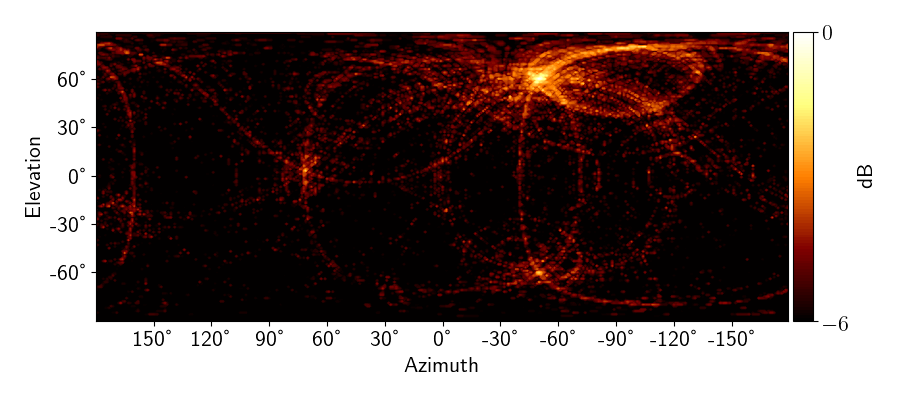
\includegraphics[width=0.8\textwidth]{Figures/Dep4mic1srcResNeg10LowDyn.png}
%\end{subfigure}
%\caption{Figures depict from SRP-PHAT localization results with SNR = -10dB, for independent microphone pairs (top), and for all  microphone pairs (bottom)}
%\label{fig:4mic1srcRedun}
%\end{figure}